\chapter[Progettazione di Sistemi e API]{Progettazione di Sistemi Software e API: dalla Traccia alla Soluzione}

Nella Sezione A, oltre ai temi discorsivi, il Settore Informazione prevede una \textbf{prova pratica di progettazione}: viene descritto un sistema reale (per esempio un cinema multisala) e si chiede di progettarne database, backend, API, diagrammi UML e un eventuale modulo di Machine Learning, \emph{rispondendo a tutti i punti}. Questo capitolo raccoglie gli strumenti e, nell'ultima parte, svolge per intero la traccia \textbf{A3-INF-4 della prima sessione 2026}.

\section{Come Affrontare la Prova Pratica}

\subsection{Metodo in sei passi}
\begin{enumerate}
    \item \textbf{Leggere tutta la traccia} e sottolineare nomi (candidati entità), verbi (operazioni e API), vincoli espliciti (``il sistema deve impedire\ldots'') e componenti già dati (per esempio ``l'interfaccia Web si assume già realizzata'').
    \item \textbf{Dichiarare le assunzioni} in poche righe: dove la traccia è ambigua, scegliere e scrivere la scelta. Le assunzioni ragionevoli e dichiarate sono valutate positivamente.
    \item \textbf{Rispondere nell'ordine dei punti numerati}, con la stessa numerazione della traccia.
    \item \textbf{Un diagramma o un codice per ogni punto che lo richiede}: se si chiede ``diagramma ER'', ``SQL'' o ``UML'', serve proprio quello, non una descrizione.
    \item \textbf{Motivare le scelte} (``scelgo X perché\ldots, alternativa Y scartata perché\ldots'').
    \item \textbf{Rileggere i vincoli}: ogni vincolo della traccia deve avere un meccanismo che lo fa rispettare (vedi l'impossibilità di prenotare due volte lo stesso posto) e va indicato esplicitamente.
\end{enumerate}

\subsection{Cosa mostrare}
\begin{itemize}
    \item Un \textbf{modello dei dati} coerente: chiavi, cardinalità, vincoli di integrità.
    \item \textbf{Separazione delle responsabilità}: livelli, componenti, interfacce.
    \item \textbf{Gestione degli errori e della concorrenza}: cosa succede se due utenti agiscono insieme o una richiesta fallisce a metà.
    \item \textbf{Sicurezza di base}: autenticazione, autorizzazione, validazione dell'input, HTTPS.
    \item \textbf{Qualità non funzionali}: scalabilità, affidabilità, manutenibilità (vedi capitolo \emph{Sistemi Distribuiti}).
\end{itemize}

\section{Progettazione di API REST}
\textbf{REST} (\emph{Representational State Transfer}) è uno stile architetturale per servizi su HTTP. Un servizio che lo rispetta si dice \emph{RESTful}.

\subsection{Principi}
\begin{itemize}
    \item \textbf{Risorse}: ogni concetto del dominio (film, proiezione, prenotazione) è una risorsa identificata da un \textbf{URL}. Gli URL contengono \emph{nomi}, non verbi: \texttt{/prenotazioni/17}, non \texttt{/creaPrenotazione}.
    \item \textbf{Interfaccia uniforme}: le operazioni sono i metodi HTTP standard.
    \item \textbf{Stateless}: ogni richiesta contiene tutto ciò che serve (compresa l'autenticazione, tipicamente un token). Il server non conserva lo stato di sessione, quindi si può replicare facilmente dietro un load balancer.
    \item \textbf{Rappresentazioni}: la stessa risorsa può avere formati diversi; oggi quasi sempre \textbf{JSON}.
    \item \textbf{Cacheabilità} delle risposte \texttt{GET} e \textbf{sistema a livelli} (gateway, proxy, load balancer trasparenti al client).
\end{itemize}

\subsection{Metodi HTTP}
\begin{center}
\small
\begin{tabularx}{\textwidth}{@{}lXlll@{}}
\toprule
\textbf{Metodo} & \textbf{Uso} & \textbf{Sicuro} & \textbf{Idempotente} & \textbf{Successo tipico} \\
\midrule
GET & Legge una risorsa o una collezione & Sì & Sì & 200 \\
POST & Crea una risorsa o avvia un'azione & No & No & 201 + \texttt{Location} \\
PUT & Sostituisce interamente una risorsa & No & Sì & 200 / 204 \\
PATCH & Modifica parziale & No & Non garantito & 200 / 204 \\
DELETE & Elimina (o annulla) una risorsa & No & Sì & 204 \\
\bottomrule
\end{tabularx}
\end{center}
\emph{Sicuro} = non modifica lo stato sul server. \emph{Idempotente} = ripetere la richiesta $n$ volte ha lo stesso effetto di una sola volta.

\subsection{Codici di stato}
\begin{itemize}
    \item \textbf{2xx successo}: 200 OK, 201 Created, 204 No Content.
    \item \textbf{3xx}: 301/302 redirect, 304 Not Modified (cache).
    \item \textbf{4xx errore del client}: 400 Bad Request (richiesta malformata), 401 Unauthorized (non autenticato), 403 Forbidden (autenticato ma non autorizzato), 404 Not Found, \textbf{409 Conflict} (conflitto con lo stato della risorsa: per esempio posto già occupato), 422 Unprocessable Entity (sintassi corretta ma dati semanticamente non validi), 429 Too Many Requests.
    \item \textbf{5xx errore del server}: 500 Internal Server Error, 503 Service Unavailable.
\end{itemize}

\subsection{Buone pratiche}
\begin{itemize}
    \item \textbf{Naming}: sostantivi al plurale, gerarchie per le relazioni di appartenenza (\texttt{/proiezioni\allowbreak/42\allowbreak/posti}).
    \item \textbf{Filtri, ordinamento, paginazione}: tramite query string (\texttt{?data=2026-11-10\&\allowbreak film=7\&\allowbreak page=2\&\allowbreak size=20}).
    \item \textbf{Versionamento}: \texttt{/api/v1/\ldots}, per poter evolvere senza rompere i client.
    \item \textbf{Formato d'errore uniforme}: per esempio \texttt{\{"errore":\allowbreak "POSTO\_OCCUPATO",\allowbreak "dettaglio":\allowbreak "\ldots"\}}.
    \item \textbf{Idempotenza delle creazioni}: l'header \texttt{Idempotency-Key} permette di ripetere un \texttt{POST} (per esempio dopo un timeout) senza creare duplicati.
    \item \textbf{Sicurezza}: HTTPS, autenticazione con token (OAuth 2 / JWT), controllo dei permessi per ruolo (utente, gestore), validazione e sanificazione dell'input, rate limiting. L'identità dell'utente si ricava dal token, \emph{non} dal corpo della richiesta.
    \item \textbf{Documentazione}: specifica \textbf{OpenAPI} (Swagger).
\end{itemize}

\subsection{REST, SOAP e gRPC}
\begin{center}
\small
\begin{tabularx}{\textwidth}{@{}lXXX@{}}
\toprule
 & \textbf{REST} & \textbf{SOAP} & \textbf{gRPC} \\
\midrule
Formato & JSON (o altro) su HTTP & XML su HTTP & Protocol Buffers su HTTP/2 \\
Stile & Risorse e metodi HTTP & Operazioni (RPC) con contratto WSDL & Chiamate remote tipizzate \\
Pro & Semplice, diffuso, cacheabile & Standard enterprise, transazioni e sicurezza avanzate & Molto efficiente, streaming \\
Uso tipico & API pubbliche, Web e mobile & Integrazione legacy aziendale & Comunicazione tra microservizi \\
\bottomrule
\end{tabularx}
\end{center}

\section{Architettura del Backend}

\subsection{Architettura a livelli}
La struttura più comune e facile da giustificare è a \textbf{tre livelli logici} dentro il backend:
\begin{itemize}
    \item \textbf{Controller / API layer}: riceve le richieste HTTP, valida il formato, autentica e autorizza, traduce JSON in oggetti e risponde con il codice di stato corretto. \emph{Non} contiene logica di business.
    \item \textbf{Service / livello di dominio}: implementa le regole di business (``una prenotazione contiene almeno un posto'', ``non si prenota una proiezione passata'') e coordina le transazioni.
    \item \textbf{Repository / accesso ai dati}: unico punto che parla con il database (SQL o ORM).
\end{itemize}
Accanto a questi: \textbf{client verso servizi esterni} (per esempio il servizio di ML), \textbf{autenticazione}, \textbf{logging e monitoraggio}, \textbf{gestione della configurazione}.

\subsection{Pattern utili}
\begin{itemize}
    \item \textbf{Repository}: incapsula l'accesso ai dati dietro un'interfaccia; si può sostituire il database nei test.
    \item \textbf{DTO} (\emph{Data Transfer Object}): oggetti usati solo per lo scambio dati con i client, separati dal modello di dominio.
    \item \textbf{Dependency Injection}: i componenti ricevono le dipendenze dall'esterno; semplifica test e sostituzione.
    \item \textbf{Facade / Gateway}: un unico punto di ingresso verso sottosistemi esterni (per esempio il modulo di ML).
    \item \textbf{MVC}: Model--View--Controller, per separare dati, presentazione e controllo.
\end{itemize}

\subsection{Integrare un modulo esterno (per esempio ML)}
\begin{itemize}
    \item Il modulo di ML è un \textbf{servizio separato} con la propria API (\texttt{POST /predizioni}); il backend lo chiama tramite un client dedicato. Vantaggi: tecnologie diverse (Python per ML), scalabilità e rilascio indipendenti, il guasto del servizio ML non blocca le prenotazioni.
    \item L'\textbf{addestramento} (offline, periodico) è separato dalla \textbf{predizione} (online o in batch); i dati sono letti da una copia o da una vista del database, per non appesantire il database transazionale.
    \item Le chiamate al servizio vanno protette con \textbf{timeout} e un \textbf{valore di ripiego} (\emph{fallback}).
\end{itemize}

\section{Concorrenza e Integrità: Evitare le Doppie Prenotazioni}
Quando due utenti prenotano lo stesso posto quasi contemporaneamente si verifica una \textbf{race condition}. Un controllo ``leggo i posti liberi, poi inserisco'' non basta: tra la lettura e la scrittura l'altro utente può inserire lo stesso posto (problema \emph{check-then-act}).

\begin{center}
\small
\begin{tabularx}{\textwidth}{@{}>{\raggedright\arraybackslash}p{3.3cm}XX@{}}
\toprule
\textbf{Tecnica} & \textbf{Come funziona} & \textbf{Note} \\
\midrule
\textbf{Vincolo di unicità} (chiave primaria o \texttt{UNIQUE}) sul biglietto & Il database rifiuta il secondo inserimento dello stesso (proiezione, posto) & \textbf{Soluzione di base, la più robusta}: la garanzia sta nel database, vale anche con più istanze del backend \\
Transazione con isolamento adeguato & Inserimento della prenotazione e dei biglietti in un'unica transazione ACID: o tutto o niente & Evita prenotazioni parziali; da sola non basta se manca il vincolo \\
Lock pessimistico (\texttt{SELECT \ldots{} FOR UPDATE}) & Blocca le righe dei posti finché la transazione non termina & Corretto, ma riduce la concorrenza e può causare deadlock se i posti non sono sempre bloccati nello stesso ordine \\
Lock ottimistico (colonna \texttt{versione}) & Si aggiorna solo se la versione non è cambiata; altrimenti si riprova & Adatto quando i conflitti sono rari \\
Blocco temporaneo (\emph{hold}) con scadenza & Il posto è riservato per alcuni minuti durante il pagamento; poi torna libero & Migliora l'esperienza utente; richiede un job di pulizia o TTL (per esempio cache con scadenza) \\
\bottomrule
\end{tabularx}
\end{center}

\paragraph{Ordine di risposta consigliato.} (1) vincolo di unicità nel database come garanzia finale; (2) transazione per atomicità; (3) il backend traduce la violazione del vincolo in risposta \textbf{409 Conflict}; (4) opzionale: hold temporaneo e verifica preliminare dei posti per un messaggio d'errore chiaro; (5) lock pessimistico solo se serve.

\paragraph{Livelli di isolamento.}
\begin{itemize}
    \item \texttt{READ COMMITTED}: evita le letture sporche.
    \item \texttt{REPEATABLE READ} e \texttt{SERIALIZABLE}: evitano anche anomalie come le \emph{non-repeatable read} e i \emph{phantom}.
    \item Con un vincolo di unicità basta in genere \texttt{READ COMMITTED}.
\end{itemize}

\section{Diagrammi UML per il Flusso Applicativo}
\begin{itemize}
    \item \textbf{Diagramma di sequenza}: mostra \emph{chi chiama chi e in quale ordine} nel tempo. È il diagramma giusto per ``il flusso di creazione di una prenotazione, dalla richiesta fino alla registrazione nel database''. Le \textbf{linee di vita} sono verticali, le frecce piene sono chiamate sincrone, quelle tratteggiate sono risposte; i frammenti \texttt{alt} (alternativa), \texttt{opt} (opzionale) e \texttt{loop} descrivono rami e cicli.
    \item \textbf{Diagramma delle attività}: mostra il flusso di controllo con decisioni e parallelismo; adatto a descrivere una procedura di business.
    \item \textbf{Diagramma dei componenti} e \textbf{di deployment}: mostrano i blocchi del sistema (Web, backend, database, servizio ML) e dove vengono eseguiti.
    \item \textbf{Diagramma delle classi}: struttura statica del dominio.
\end{itemize}
Per gli aspetti generali di UML si veda il capitolo \emph{Progettazione del Software}.

\section{Tema Svolto: Cinema Multisala (A3-INF-4, 2026)}
\textbf{Sintesi della traccia.} Un cinema multisala vuole un sistema per consultare la programmazione, prenotare posti e pianificare le proiezioni future. Componenti: interfaccia Web (già realizzata), backend applicativo, base di dati relazionale, modulo di Machine Learning. Un film ha più proiezioni (sala, data e ora, prezzo); una sala ha posti identificati da fila e numero; gli utenti sono già registrati, scelgono una proiezione e prenotano uno o più posti; \textbf{lo stesso posto non può essere prenotato due volte per la stessa proiezione}. Il modulo di ML stima la domanda delle future proiezioni. La prova richiede di svolgere \emph{tutti} i 9 punti, divisi in tre parti.

\paragraph{Assunzioni dichiarate.}
(i) Gli utenti sono già registrati e autenticati con un token. (ii) Il pagamento è fuori dall'ambito: una prenotazione si considera confermata alla creazione. (iii) Un posto appartiene a una sola sala e ogni proiezione si svolge in una sola sala. (iv) Il prezzo è unico per proiezione. (v) Il gestore è un ruolo distinto dall'utente.

\subsection{Parte 1: progettazione della base di dati}

\subsubsection*{Punto 1 -- Modello concettuale (ER)}
\begin{figure}[h!]
    \centering
    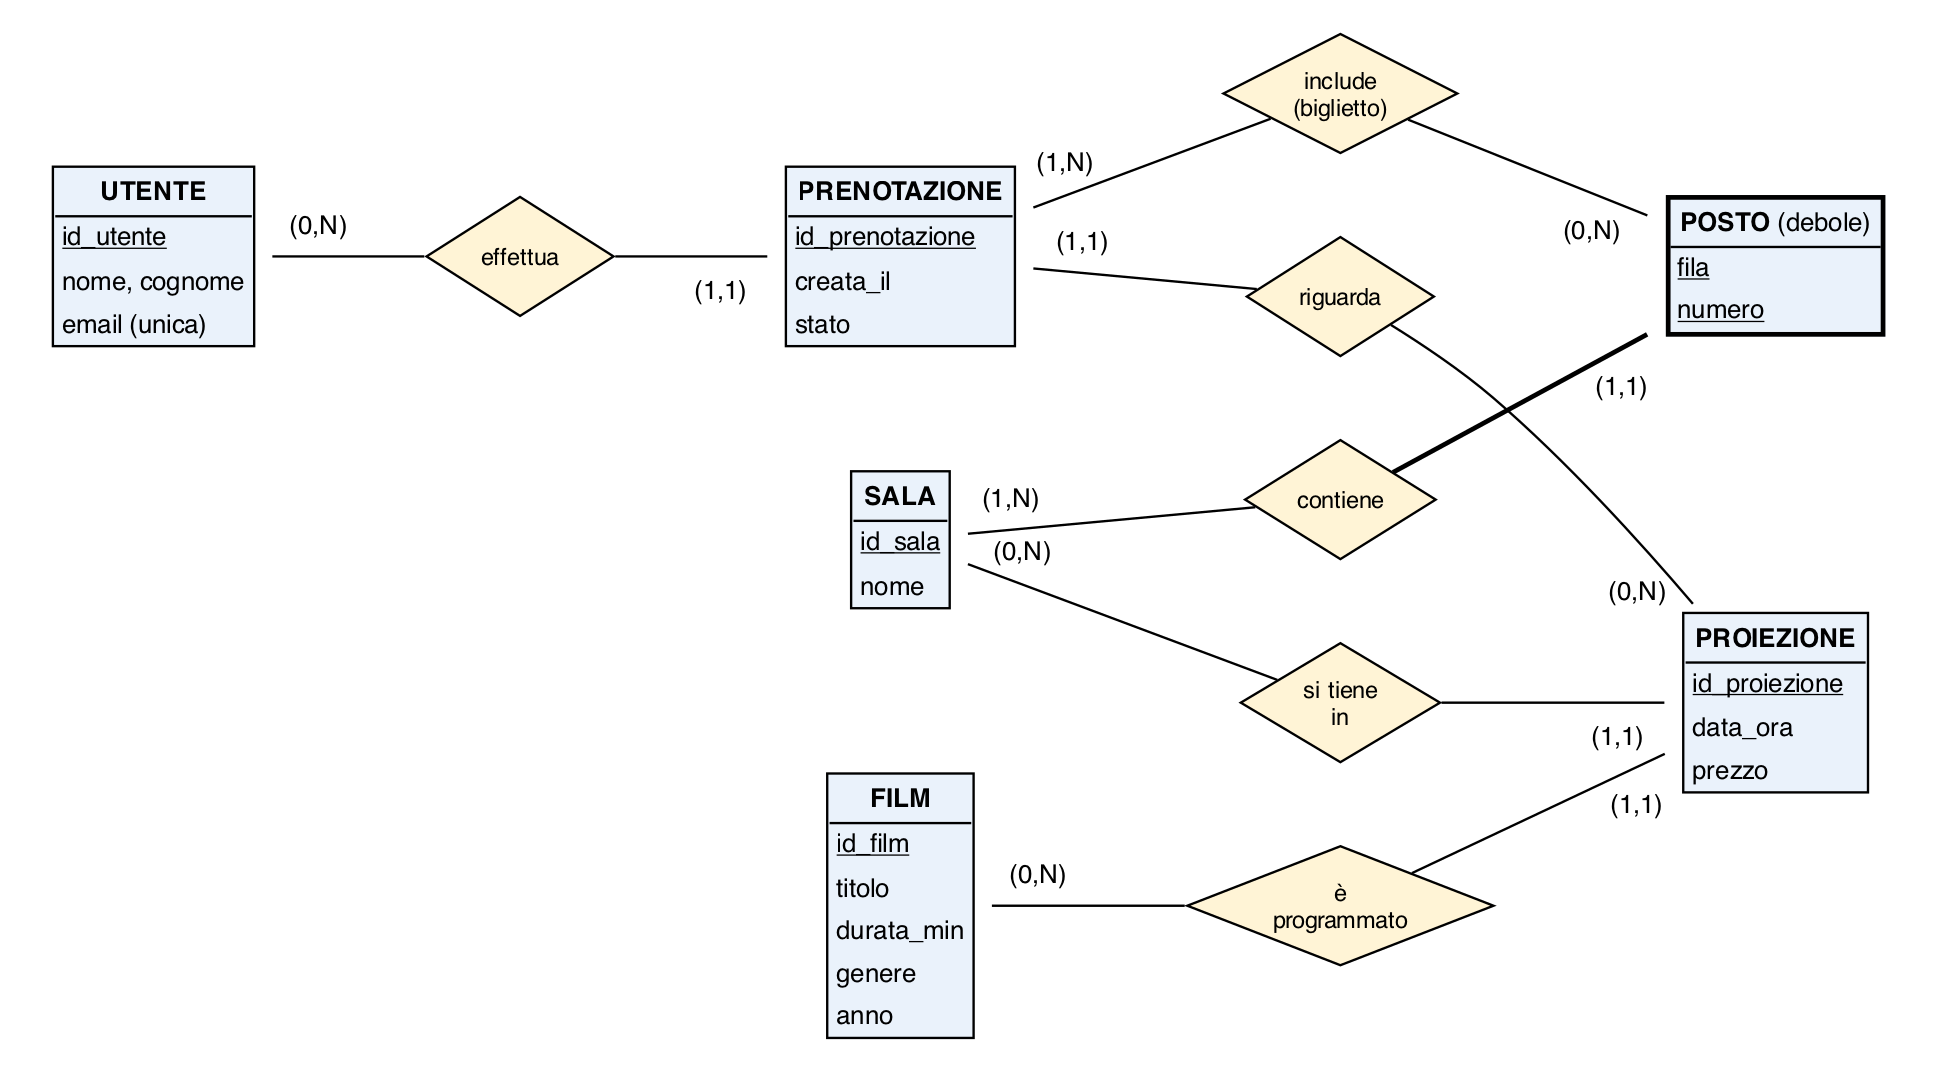
\includegraphics[width=\textwidth]{immagini/er_cinema_multisala.png}
    \caption{Schema ER del cinema multisala. Le cardinalità $(min,max)$ sono scritte accanto all'entità a cui si riferiscono.}
    \label{fig:er_cinema}
\end{figure}

\textbf{Entità e attributi principali}
\begin{itemize}
    \item \textbf{FILM}(\underline{id\_film}, titolo, durata\_min, genere, anno).
    \item \textbf{SALA}(\underline{id\_sala}, nome).
    \item \textbf{POSTO}(fila, numero) -- \textbf{entità debole} di SALA: identificata da (id\_sala, fila, numero), perché ``fila C, numero 7'' esiste in ogni sala.
    \item \textbf{PROIEZIONE}(\underline{id\_proiezione}, data\_ora, prezzo).
    \item \textbf{UTENTE}(\underline{id\_utente}, nome, cognome, email unica).
    \item \textbf{PRENOTAZIONE}(\underline{id\_prenotazione}, creata\_il, stato).
\end{itemize}

\textbf{Associazioni e cardinalità}
\begin{itemize}
    \item FILM $(0,N)$ -- \emph{è programmato} -- $(1,1)$ PROIEZIONE: un film può avere molte proiezioni (o nessuna); ogni proiezione è di un solo film.
    \item SALA $(0,N)$ -- \emph{si tiene in} -- $(1,1)$ PROIEZIONE.
    \item SALA $(1,N)$ -- \emph{contiene} -- $(1,1)$ POSTO (identificazione esterna).
    \item UTENTE $(0,N)$ -- \emph{effettua} -- $(1,1)$ PRENOTAZIONE.
    \item PRENOTAZIONE $(1,1)$ -- \emph{riguarda} -- $(0,N)$ PROIEZIONE.
    \item PRENOTAZIONE $(1,N)$ -- \emph{include} (con la proiezione: \emph{biglietto}) -- $(0,N)$ POSTO: una prenotazione contiene uno o più posti. Il biglietto lega prenotazione, proiezione e posto.
\end{itemize}

\textbf{Vincoli significativi (non esprimibili nel solo diagramma)}
\begin{enumerate}
    \item \textbf{Un posto non può essere prenotato due volte per la stessa proiezione}: la coppia (proiezione, posto) compare al più in un biglietto.
    \item Il posto prenotato deve appartenere alla \textbf{sala in cui si tiene la proiezione}.
    \item I posti di una prenotazione si riferiscono alla \emph{stessa} proiezione della prenotazione.
    \item Due proiezioni nella stessa sala non possono avere la stessa data e ora (e, volendo, non si devono sovrapporre).
    \item Il prezzo non è negativo; l'email dell'utente è unica.
\end{enumerate}

\subsubsection*{Punto 2 -- Modello relazionale}
Le chiavi primarie sono sottolineate, le chiavi esterne indicate con $\rightarrow$.

\begin{itemize}
    \item FILM(\underline{id\_film}, titolo, durata\_min, genere, anno)
    \item SALA(\underline{id\_sala}, nome)
    \item POSTO(\underline{id\_sala}$\rightarrow$SALA, \underline{fila}, \underline{numero})
    \item PROIEZIONE(\underline{id\_proiezione}, id\_film$\rightarrow$FILM, id\_sala$\rightarrow$SALA, data\_ora, prezzo)\\
          \emph{Chiavi candidate}: (id\_sala, data\_ora) e (id\_proiezione, id\_sala).
    \item UTENTE(\underline{id\_utente}, nome, cognome, email)
    \item PRENOTAZIONE(\underline{id\_prenotazione}, id\_utente$\rightarrow$UTENTE, id\_proiezione$\rightarrow$PROIEZIONE, creata\_il, stato)\\
          \emph{Chiave candidata}: (id\_prenotazione, id\_proiezione).
    \item BIGLIETTO(\underline{id\_proiezione}, \underline{fila}, \underline{numero}, id\_prenotazione, id\_sala)\\
          \emph{Chiavi esterne}:\\
          (id\_prenotazione, id\_proiezione)$\rightarrow$PRENOTAZIONE;\\
          (id\_proiezione, id\_sala)$\rightarrow$PROIEZIONE;\\
          (id\_sala, fila, numero)$\rightarrow$POSTO.
\end{itemize}

\textbf{Come i vincoli sono garantiti}
\begin{itemize}
    \item Il vincolo 1 è garantito dalla \textbf{chiave primaria} (id\_proiezione, fila, numero) di BIGLIETTO: lo stesso posto non può comparire due volte per la stessa proiezione, \emph{qualunque sia il numero di istanze del backend}.
    \item I vincoli 2 e 3 sono garantiti dalle \textbf{chiavi esterne composte}: il biglietto referenzia la coppia (id\_proiezione, id\_sala) di PROIEZIONE e il posto (id\_sala, fila, numero) di POSTO, quindi il posto deve appartenere alla sala della proiezione; referenzia la coppia (id\_prenotazione, id\_proiezione) di PRENOTAZIONE.
    \item Il vincolo 4 con \texttt{UNIQUE (id\_sala, data\_ora)}; il 5 con \texttt{CHECK} e \texttt{UNIQUE}.
\end{itemize}

\subsubsection*{Punto 3 -- SQL}
\begin{lstlisting}[language=SQL, caption={Creazione delle tabelle (sintassi in stile PostgreSQL)}]
CREATE TABLE film (
  id_film     INTEGER PRIMARY KEY,
  titolo      VARCHAR(200) NOT NULL,
  durata_min  INTEGER NOT NULL CHECK (durata_min > 0),
  genere      VARCHAR(50),
  anno        INTEGER
);

CREATE TABLE sala (
  id_sala  INTEGER PRIMARY KEY,
  nome     VARCHAR(50) NOT NULL UNIQUE
);

CREATE TABLE posto (
  id_sala  INTEGER NOT NULL REFERENCES sala(id_sala),
  fila     CHAR(1) NOT NULL,
  numero   INTEGER NOT NULL CHECK (numero > 0),
  PRIMARY KEY (id_sala, fila, numero)
);

CREATE TABLE proiezione (
  id_proiezione  INTEGER PRIMARY KEY,
  id_film        INTEGER NOT NULL REFERENCES film(id_film),
  id_sala        INTEGER NOT NULL REFERENCES sala(id_sala),
  data_ora       TIMESTAMP NOT NULL,
  prezzo         DECIMAL(6,2) NOT NULL CHECK (prezzo >= 0),
  UNIQUE (id_sala, data_ora),
  UNIQUE (id_proiezione, id_sala)
);

CREATE TABLE utente (
  id_utente  INTEGER PRIMARY KEY,
  nome       VARCHAR(50) NOT NULL,
  cognome    VARCHAR(50) NOT NULL,
  email      VARCHAR(120) NOT NULL UNIQUE
);

CREATE TABLE prenotazione (
  id_prenotazione  INTEGER PRIMARY KEY,
  id_utente        INTEGER NOT NULL REFERENCES utente(id_utente),
  id_proiezione    INTEGER NOT NULL REFERENCES proiezione(id_proiezione),
  creata_il        TIMESTAMP NOT NULL DEFAULT CURRENT_TIMESTAMP,
  stato            VARCHAR(12) NOT NULL DEFAULT 'CONFERMATA'
                   CHECK (stato IN ('CONFERMATA', 'ANNULLATA')),
  UNIQUE (id_prenotazione, id_proiezione)
);

CREATE TABLE biglietto (
  id_proiezione    INTEGER NOT NULL,
  fila             CHAR(1) NOT NULL,
  numero           INTEGER NOT NULL,
  id_prenotazione  INTEGER NOT NULL,
  id_sala          INTEGER NOT NULL,
  -- un posto non puo' essere venduto due volte per la stessa proiezione
  PRIMARY KEY (id_proiezione, fila, numero),
  FOREIGN KEY (id_prenotazione, id_proiezione)
      REFERENCES prenotazione(id_prenotazione, id_proiezione),
  -- la proiezione si tiene in quella sala...
  FOREIGN KEY (id_proiezione, id_sala)
      REFERENCES proiezione(id_proiezione, id_sala),
  -- ...e il posto appartiene a quella sala
  FOREIGN KEY (id_sala, fila, numero)
      REFERENCES posto(id_sala, fila, numero)
);
\end{lstlisting}

\begin{lstlisting}[language=SQL, caption={Posti ancora disponibili per una proiezione}]
SELECT p.fila, p.numero
FROM proiezione pr
JOIN posto p ON p.id_sala = pr.id_sala
WHERE pr.id_proiezione = :id_proiezione
  AND NOT EXISTS (
    SELECT 1
    FROM biglietto b
    WHERE b.id_proiezione = pr.id_proiezione
      AND b.fila   = p.fila
      AND b.numero = p.numero
  )
ORDER BY p.fila, p.numero;
\end{lstlisting}
La query prende i posti della sala in cui si tiene la proiezione e scarta quelli che compaiono tra i biglietti della stessa proiezione (\texttt{NOT EXISTS}, \emph{anti-join}). Un'alternativa equivalente usa \texttt{LEFT JOIN \ldots{} WHERE b.fila IS NULL}. Con la chiave primaria di BIGLIETTO, la ricerca per proiezione usa già l'indice.

\paragraph{Nota.} L'annullamento di una prenotazione deve \textbf{liberare i posti}: si eliminano i suoi biglietti (eventualmente copiandoli prima in una tabella di storico) e si pone lo stato a \texttt{ANNULLATA}.

\subsection{Parte 2: progettazione del backend}

\subsubsection*{Punto 4 -- Componenti logici e interazioni}
\begin{center}
\small
\begin{tabularx}{\textwidth}{@{}>{\raggedright\arraybackslash}p{3.4cm}XX@{}}
\toprule
\textbf{Componente} & \textbf{Responsabilità} & \textbf{Interazioni} \\
\midrule
API / Controller & Espone gli endpoint REST, valida l'input, autentica (token) e autorizza per ruolo, traduce errori in codici HTTP & Riceve le richieste dall'interfaccia Web; chiama i servizi \\
Servizio Programmazione & Elenca film e proiezioni, filtri per data e film & Legge dal database tramite repository \\
Servizio Prenotazioni & Calcola i posti disponibili, crea e annulla prenotazioni con le regole di business e la transazione & Usa il repository; \textbf{unico punto che scrive prenotazioni e biglietti} \\
Repository / DAO & Accesso al database relazionale (SQL), mappatura tra tabelle e oggetti & Database \\
Servizio Previsioni (client ML) & Prepara le richieste per il modulo di ML, chiama il suo servizio, applica timeout e valori di ripiego, espone i risultati al gestore & Modulo di Machine Learning; database per i dati storici \\
Autenticazione e autorizzazione & Verifica il token e il ruolo (utente o gestore) & Usato dal controller \\
Logging e monitoraggio & Registra richieste ed errori, metriche & Trasversale \\
\bottomrule
\end{tabularx}
\end{center}

\textbf{Flusso di una richiesta}: interfaccia Web $\to$ Controller $\to$ Servizio $\to$ Repository $\to$ Database, e risposta lungo il percorso inverso. Il modulo ML è un servizio separato: il backend lo chiama \emph{solo} per le funzioni del gestore, \emph{mai} nel percorso critico della prenotazione, così un guasto del modulo ML non blocca i clienti.

\subsubsection*{Punto 5 -- API}
\begin{center}
\small
\begin{tabularx}{\textwidth}{@{}>{\raggedright\arraybackslash}p{1.3cm}>{\raggedright\arraybackslash}p{4.6cm}Xl@{}}
\toprule
\textbf{Metodo} & \textbf{Endpoint} & \textbf{Descrizione} & \textbf{Esiti} \\
\midrule
GET & \texttt{/api/v1/film} & Elenco film (filtri: data, genere) & 200 \\
GET & \texttt{/api/v1/proiezioni?data=\&film=} & Programmazione: proiezioni filtrate per data e film, con sala, orario, prezzo & 200, 400 \\
GET & \texttt{/api/v1/proiezioni/\{id\}} & Dettaglio di una proiezione & 200, 404 \\
GET & \texttt{/api/v1/proiezioni/\{id\}/posti} & Posti con stato \emph{libero/occupato} & 200, 404 \\
POST & \texttt{/api/v1/proiezioni/\{id\}/prenotazioni} & Crea una prenotazione per uno o più posti & 201, 400, 401, 404, \textbf{409}, 422 \\
GET & \texttt{/api/v1/prenotazioni/\{id\}} & Dettaglio di una prenotazione dell'utente & 200, 403, 404 \\
DELETE & \texttt{/api/v1/prenotazioni/\{id\}} & Annulla e libera i posti & 204, 403, 404 \\
GET & \texttt{/api/v1/gestore/previsioni?da=\&a=} & Previsioni di domanda (ruolo gestore) & 200, 403, 503 \\
\bottomrule
\end{tabularx}
\end{center}

\begin{lstlisting}[numbers=none, caption={Esempio: elenco dei posti di una proiezione}]
GET /api/v1/proiezioni/42/posti

200 OK
{
  "id_proiezione": 42,
  "sala": "Sala 3",
  "prezzo": 9.50,
  "posti": [
    { "fila": "A", "numero": 1, "stato": "libero" },
    { "fila": "A", "numero": 2, "stato": "occupato" }
  ]
}
\end{lstlisting}

\begin{lstlisting}[numbers=none, caption={Esempio: creazione di una prenotazione}]
POST /api/v1/proiezioni/42/prenotazioni
Authorization: Bearer <token>
Idempotency-Key: 3f2a-...
{ "posti": [ { "fila": "C", "numero": 7 }, { "fila": "C", "numero": 8 } ] }

201 Created
Location: /api/v1/prenotazioni/1017
{ "id_prenotazione": 1017, "id_proiezione": 42, "totale": 19.00,
  "posti": [ { "fila": "C", "numero": 7 }, { "fila": "C", "numero": 8 } ] }

409 Conflict   (posto gia' occupato)
{ "errore": "POSTO_OCCUPATO", "posti": [ { "fila": "C", "numero": 7 } ] }
\end{lstlisting}

\paragraph{Scelte progettuali.} L'identità dell'utente deriva dal \emph{token}, non dal corpo della richiesta. L'\texttt{Idempotency-Key} evita prenotazioni doppie se il client ripete la richiesta dopo un timeout. Le risposte \texttt{GET} sui posti non sono cacheabili a lungo, perché cambiano di continuo (e la disponibilità letta non è una garanzia: l'unica garanzia è l'inserimento).

\begin{lstlisting}[language=Python, caption={Pseudocodice del servizio di prenotazione (stile Python)}]
def crea_prenotazione(db, id_utente, id_proiezione, posti):
    if not posti:
        raise RichiestaNonValida("almeno un posto")
    with db.transazione():                         # BEGIN ... COMMIT/ROLLBACK
        pr = db.una_riga("SELECT id_sala, data_ora FROM proiezione "
                         "WHERE id_proiezione = %s", id_proiezione)
        if pr is None:
            raise NonTrovato()                     # -> 404
        if pr.data_ora < adesso():
            raise RichiestaNonValida("proiezione passata")   # -> 422
        id_pren = db.scalare(
            "INSERT INTO prenotazione (id_utente, id_proiezione) "
            "VALUES (%s, %s) RETURNING id_prenotazione",
            id_utente, id_proiezione)
        try:
            for fila, numero in sorted(posti):     # ordine fisso: niente deadlock
                db.esegui(
                    "INSERT INTO biglietto "
                    "(id_proiezione, fila, numero, id_prenotazione, id_sala) "
                    "VALUES (%s, %s, %s, %s, %s)",
                    id_proiezione, fila, numero, id_pren, pr.id_sala)
        except ViolazioneUnicita:                  # chiave primaria del biglietto
            raise PostoOccupato()                  # rollback automatico -> 409
        except ViolazioneChiaveEsterna:            # posto inesistente nella sala
            raise RichiestaNonValida("posto non valido")     # -> 422
    return id_pren
\end{lstlisting}

\subsubsection*{Punto 6 -- Diagramma di sequenza e prevenzione dei doppioni}
\begin{figure}[h!]
    \centering
    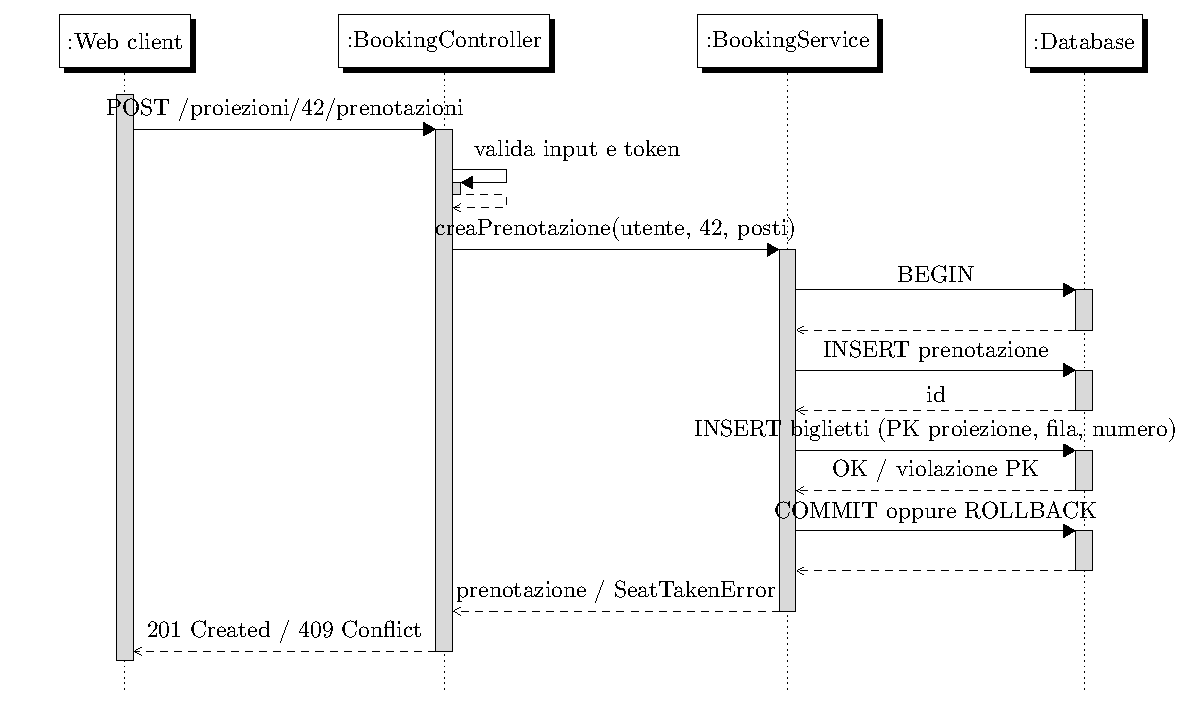
\includegraphics[width=\textwidth]{immagini/uml_sequence_prenotazione_cinema.png}
    \caption{Diagramma di sequenza della creazione di una prenotazione.}
    \label{fig:seq_prenotazione}
\end{figure}

\textbf{Flusso}
\begin{enumerate}
    \item L'interfaccia Web invia \texttt{POST /proiezioni/42/prenotazioni} con il token e i posti scelti.
    \item Il controller valida il formato e il token e chiama il servizio.
    \item Il servizio \textbf{apre una transazione}, inserisce la prenotazione e inserisce un biglietto per ogni posto.
    \item Se tutti gli inserimenti riescono, la transazione fa \textbf{COMMIT} e il controller risponde \textbf{201 Created}.
    \item Se un inserimento viola la chiave primaria (posto già venduto per quella proiezione), la transazione fa \textbf{ROLLBACK} (nessuna prenotazione parziale) e il controller risponde \textbf{409 Conflict}.
\end{enumerate}

\textbf{Operazioni che impediscono la doppia assegnazione}
\begin{itemize}
    \item \textbf{Vincolo di unicità} (chiave primaria del biglietto): è la garanzia vera, perché è valutata dal database in modo atomico anche con più richieste concorrenti. Se due utenti prenotano lo stesso posto nello stesso istante, uno solo vince.
    \item \textbf{Transazione}: prenotazione e biglietti sono scritti insieme o per nulla.
    \item \textbf{Ordine fisso} dei posti negli inserimenti, per evitare deadlock tra richieste che toccano insiemi di posti sovrapposti.
    \item \textbf{Alternativa}: lock pessimistico (\texttt{SELECT \ldots{} FOR UPDATE}) sui posti, oppure \emph{hold} temporaneo con scadenza durante il pagamento. Non sostituiscono il vincolo ma migliorano l'esperienza utente.
    \item \textbf{Controllo preliminare} (lettura dei posti liberi) solo come cortesia per l'interfaccia: \emph{non} è una garanzia.
\end{itemize}

\subsection{Parte 3: modulo di Machine Learning}

\subsubsection*{Punto 7 -- Progetto della soluzione}
\begin{itemize}
    \item \textbf{Problema}: \textbf{regressione supervisionata}. Si hanno dati storici con l'esito reale per ogni proiezione.
    \item \textbf{Variabile da prevedere} (\emph{target}): il \textbf{numero di biglietti venduti} per proiezione, oppure il \textbf{tasso di occupazione} $=$ biglietti venduti $/$ capienza della sala (più confrontabile tra sale diverse).
    \item \textbf{Variabili di ingresso (feature)}
    \begin{itemize}
        \item \emph{Film}: genere, durata, anno di uscita, settimane dall'uscita, regista o cast o saga, giudizi o popolarità, vendite delle proiezioni precedenti dello stesso film.
        \item \emph{Tempo}: giorno della settimana, fascia oraria, festivo o prefestivo, vacanze, stagione, mese; eventuale meteo.
        \item \emph{Proiezione}: prezzo, sala e capienza, formato (3D, lingua originale).
        \item \emph{Contesto}: numero di proiezioni in concorrenza nello stesso orario, promozioni.
    \end{itemize}
    \item \textbf{Modello}: \textbf{gradient boosting su alberi} (o \emph{random forest}) come scelta principale: gestisce feature miste (numeriche e categoriche), relazioni non lineari e interazioni (giorno $\times$ ora $\times$ genere) con pochi dati e poca preparazione; è robusto e abbastanza interpretabile (importanza delle feature). Come \textbf{baseline} si usano la media storica per lo stesso giorno, ora e genere oppure una \textbf{regressione lineare}; il modello complesso va adottato solo se batte la baseline. Con molti dati si possono valutare reti neurali o modelli per serie temporali.
\end{itemize}

\subsubsection*{Punto 8 -- Addestramento e valutazione}
\begin{enumerate}
    \item \textbf{Preparazione dei dati}: estrazione dal database (proiezioni e biglietti), \textbf{pulizia} (valori mancanti, errori), codifica delle categoriche, costruzione delle feature.
    \item \textbf{Suddivisione dei dati \emph{temporale}} (non casuale): addestramento sul periodo più vecchio, validazione sul periodo successivo (scelta degli iperparametri), test sull'ultimo periodo (per esempio $70\%/15\%/15\%$ in ordine cronologico). Una suddivisione casuale farebbe ``vedere il futuro'' al modello (\emph{data leakage}) e darebbe una stima ottimistica. In alternativa, \textbf{validazione a finestre scorrevoli} (\emph{time series cross-validation}).
    \item \textbf{Addestramento}: ottimizzazione degli iperparametri sul set di validazione, \textbf{regolarizzazione} e early stopping per evitare l'overfitting.
    \item \textbf{Metriche}: \textbf{MAE} (errore medio in biglietti, facile da interpretare), \textbf{RMSE} (penalizza gli errori grandi), \textbf{WAPE/MAPE} (errore relativo; MAPE è instabile con valori prossimi a zero); confronto con la baseline. Si controlla anche l'errore per sottogruppi (sala, giorno, film nuovi).
    \item \textbf{Test finale} \emph{una sola volta} sul test set, e \textbf{monitoraggio} dopo il deployment con riaddestramento periodico.
\end{enumerate}

\subsubsection*{Punto 9 -- Uso delle predizioni e limiti}
\textbf{Come usarle per il gestore}
\begin{itemize}
    \item \textbf{Assegnazione delle sale}: abbinare la domanda stimata alla \textbf{capienza}; film con alta domanda previsto $\to$ sala grande; domanda bassa $\to$ sala piccola, per riempire le sale e non sprecare risorse.
    \item \textbf{Numero e orari delle proiezioni}: se la domanda prevista in una fascia supera la capienza, aggiungere una proiezione o spostarla in una sala maggiore; ridurre le proiezioni nelle fasce con bassa domanda.
    \item \textbf{Prezzi e promozioni}: prezzi più bassi per fasce deboli, promozioni mirate.
    \item \textbf{Uso come supporto}: si mostrano al gestore la stima e un \textbf{intervallo di incertezza}; si può formulare l'assegnazione come problema di \textbf{ottimizzazione vincolata} (sale disponibili, orari, durate dei film) con le previsioni come input.
\end{itemize}

\textbf{Limiti}
\begin{itemize}
    \item \textbf{Dati censurati}: i biglietti venduti non possono superare la capienza; se una sala si riempie, la domanda reale era maggiore. Il modello sottostima la domanda dei successi.
    \item \textbf{Circolo vizioso} (\emph{feedback loop}): se il modello assegna una sala piccola, le vendite saranno limitate e il modello ``imparerà'' che la domanda è bassa.
    \item \textbf{Film nuovi} (\emph{cold start}) senza storico; eventi imprevedibili (successi inattesi, maltempo, scioperi); \textbf{cambiamenti} nelle abitudini (\emph{drift}).
    \item \textbf{Incertezza}: le stime sono previsioni, non garanzie; l'errore va comunicato.
    \item \textbf{Decisione finale al gestore}, che conosce informazioni non nei dati; attenzione a equità e privacy dei dati degli utenti (GDPR: dati aggregati e anonimizzati).
\end{itemize}

\section{Checklist e Errori Comuni}
\begin{itemize}
    \item \textbf{Rispondere a tutti i punti} e nell'ordine; usare la stessa numerazione della traccia.
    \item \textbf{Non scrivere solo prosa} dove si chiede un diagramma, un SQL o una tabella.
    \item \textbf{Dichiarare le assunzioni} e usarle in modo coerente.
    \item \textbf{Ogni vincolo della traccia deve avere un meccanismo}: qui, il vincolo di unicità.
    \item Nel modello relazionale: \textbf{chiavi primarie ed esterne} indicate e coerenti con lo schema ER.
    \item \textbf{Non mettere logica di business nel controller} né SQL nei controller.
    \item Per le API: \textbf{nomi (non verbi)} negli URL, metodi e codici di stato corretti, 409 per i conflitti.
    \item Per il ML: \textbf{suddivisione temporale}, baseline, metrica adeguata, limiti dichiarati.
    \item \textbf{Controllare il tempo}: schemi semplici e corretti valgono più di schemi complicati e incompleti.
\end{itemize}
